\chapter{User Interface Design}\label{ch:user-interface-design}
This chapter is focused on the user interface design of the Dronetag mobile application.
It starts with an explanation of difference between UI (User Interface) and UX (User Experience), and continues with a description about the user interface structure of this application.
So, it contains a list of screens that are shown to users when the users go through the application.

The main difference between UI and UX is in the approach.
UI approach emphasizes a combination of visual elements such that the final concept of visualization fits together.
UX approach emphasizes an arrangement of these visual elements such that their arrangement was logical, and it was close to human thinking.~\cite{prototyping}
There are many visual elements.
They can be:
\begin{itemize}
    \item A text label,
    \item A text field,
    \item A button,
    \item A checkbox,
    \item A List view,
    \item A menu,
    \item An icon,
    \item An image,
    \item And others.
\end{itemize}
UI approach deals with their skin~-~for example, a color, size, shadow, border, shape, and others.
UX approach focuses on the size and position on the screen.
The arrangement of elements in screens should be comprehensive and should make sense to users.

The user interface design phase usually includes Lo-Fi (Low Fidelity) and Hi-Fi (High Fidelity) prototyping.~\cite{effectivePrototyping}
There will be clarified the difference between them.
Lo-Fi, how the name hints, is a simplified sketch without colors with a purpose to incorporate the elements on a screen together.
It is cheaper than Hi-Fi and takes only a few hours to finish.
The benefits are:
\begin{itemize}
    \item Focus on design and concepts,
    \item Focus on design and concepts,
    \item Accessible to everyone.~\cite{hiFiLoFiPrototypeArticle}
\end{itemize}

In opposite, Hi-Fi, how the name hints, includes a fidelity design that should correspond to the final product.
It is more expensive than Lo-Fi and usually takes a few days.
The benefits are:
\begin{itemize}
    \item More familiar to users,
    \item Pinpoint specific components to test,
    \item More presentable to stakeholders.~\cite{hiFiLoFiPrototypeArticle}
\end{itemize}
To more information about fidelity, anyone can read this article~\cite{hiFiLoFiPrototypeArticle}.

Lo-Fi prototype has not been created because Dronetag is Start-up, a company with a limited budget, so there is only the Hi-Fi prototype.
When Hi-Fi was being made, it was inspired by a few competitor applications, which show permitted flight zones and danger areas.
These applications are described in the Related projects chapter~\ref{ch:related-projects}, so they will not be discussed anymore.


\section{Hi-Fi Prototype}\label{sec:hi-fi-prototype}
This section consists of screens in the application with a detailed description of their elements.
The \acrshort{hifi} prototype was made by Marian Hlav{\' a}{\v c} in Adobe XD~\cite{adobeXD} and is available online~\cite{hifiPrototype}.
It was emphasized to the simplicity and briefness and kept the focus on the essential \acrshort{ui} and \acrshort{ux} design rules.
These rules are based on "Jakob Nielsen's 10 general principles for interaction design".~\cite{nnGroup}
It describes key aspects of User Interface Design.
The heuristics by Jakob Nielsen are the following:
\begin{enumerate}
    \item Visibility of system status,
    \item Match between system and the real world,
    \item User control and freedom,
    \item Consistency and standards,
    \item Error prevention,
    \item Recognition rather than recall,
    \item Flexibility and efficiency of use,
    \item Aesthetic and minimalist design,
    \item Help users recognize, diagnose, and recover from errors,
    \item Help and documentation.
\end{enumerate}

Applications built on these heuristics will be successful and useful because these heuristics are based on various psychological researches and usability testing with ordinary users.

\subsection{Dashboard}\label{subsec:dashboard2}

The Dashboard screen is immediately after the Splash screen.
It is counted on the fact users will spend most of the time on the Dashboard screen, and so it contains the main functionalities.
This screen is divided into Top panel and Map controls.
These elements are in the higher stack layer above the map where are placed flying drones, place pins and restricted areas.
Besides, it allows displaying without wasteful \acrshort{poi}s~(\acrlong{poi})~\cite{poi}, satellite map or standard map, which contains \acrshort{poi}s, precisely like Google Maps application.

The Top panel is consists of:
\begin{itemize}
    \item \textbf{Device status} - it contains current information about default device,
    \item \textbf{Search button} - it opens the Search screen for searching of places, devices, aircrafts and zones,
    \item \textbf{Profile button} - it open the Profile screen that represents the main menu of the whole application.
\end{itemize}
If a user has already logged in and planned a flight, Profile button contains a light blue circle with the number of planned flights in the top right on the circuit of that circle button.
It is able to see on the picture~\ref{fig:dashboard}.

The Map controls are consists of:
\begin{itemize}
    \item \textbf{My location button} - it redirects to his position due to his location by \acrshort{gps} coordinates,
    \item \textbf{Map layers button} - it is an offer allowing users to choose a map style,
    \item \textbf{Fly now button} - this button shows drop down menu with Fly now and Plan a flight options for already logged in users, and Log in and sign up button for unauthorized users.
\end{itemize}
\newpage
These are additional elements that are shown on the Dashboard screen:
\begin{itemize}
    \item Drone detail panel, (Figure~\ref{fig:dashboard_drone_detail})
    \item Place detail panel,
    \item Zone detail panel, (Figure~\ref{fig:dashboard_zone_detail})
    \item Zone selection panel,
    \item Map layer panel.
\end{itemize}

The Drone detail panel is for showing necessary information and a flying drone and its flight parameters.
Besides, it contains the button to redirect to the full drone detail screen, where users can see all information about live flight immediately.

The Place detail panel contains necessary information about the place.
Also, if users want to plan a flight from this place, it allows them to pin this place on the map until they unpins it and Plan a flight button.
Place pinning into the map is demonstrated by a color change of the pin on the map and icon in the panel.

The Zone detail panel contains necessary information about the given zone, such as a lower altitude level, upper altitude level, name of the zone, and validation from and zone status.

The Zone selection is used to select a zone if a user clicks to a place in the map where is an intersection of more zones.
Simultaneously, when this selection is shown, the selected zones are highlighted.
If a user chooses a zone, the zone will show Zone detail panel and it will be highlighted only the particular zone instead of the intersection.

It was focused on the primary purpose of informing users about drones and restricted areas around them.
So, it was decided to keep a minimalistic design because the users needs to emphasize to important elements to them.


\begin{figure}
    \centering
    \begin{minipage}{.4\textwidth}
        \centering
        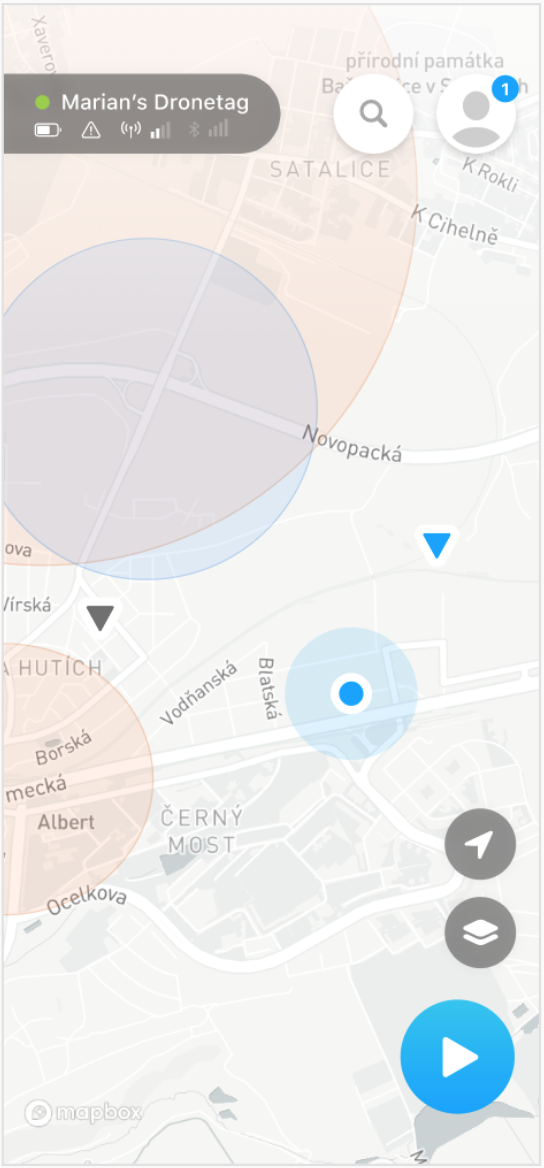
\includegraphics[width=.7\linewidth]{assets/user_interface_design/dashboard/dashboard.png}
        \caption{Dashboard}
        \label{fig:dashboard}
    \end{minipage}%
    \hspace{.05\linewidth}
    \begin{minipage}{.4\textwidth}
        \centering
        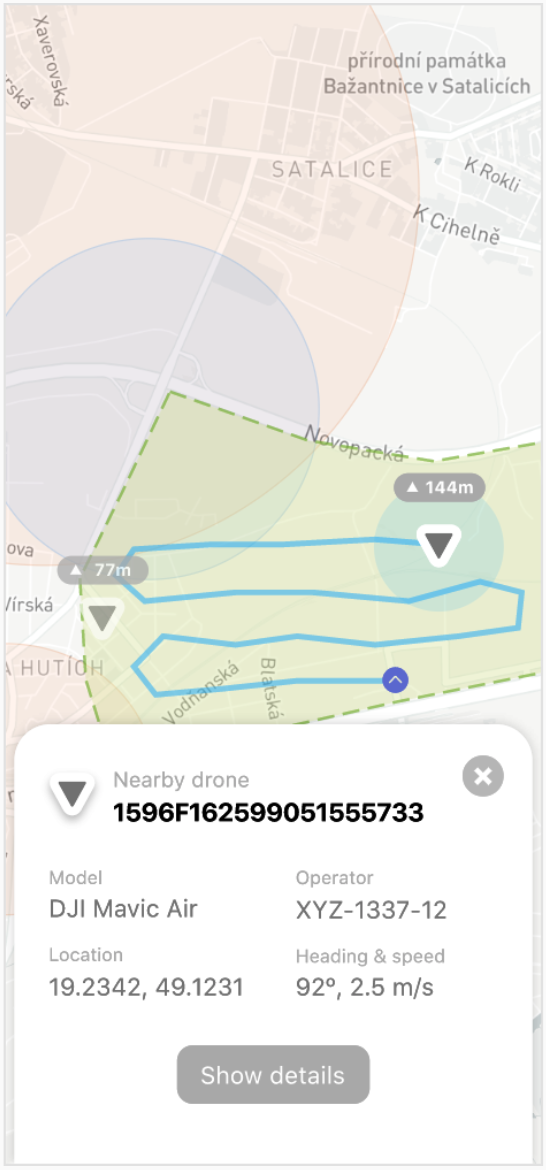
\includegraphics[width=.7\linewidth]{assets/user_interface_design/dashboard/dashboard_drone_detail.png}
        \caption{Drone detail}
        \label{fig:dashboard_drone_detail}
    \end{minipage}
    \label{fig:dashboard_all}
\end{figure}


\subsection{Login and Registration screens}\label{subsec:login-screen}
%todo: add text


\begin{figure}
    \centering
    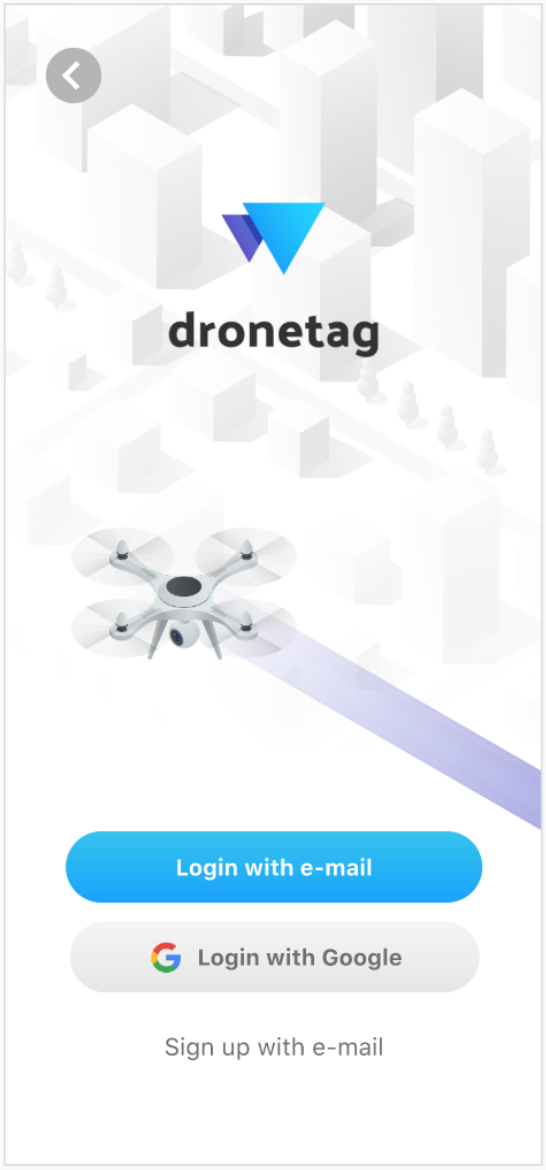
\includegraphics[width=.3\linewidth]{assets/user_interface_design/login/login_screen.png}
    \caption{[A10] Login screen}
    \label{fig:login_screen}
\end{figure}

\begin{figure}
    \centering
    \begin{minipage}{.45\textwidth}
        \centering
        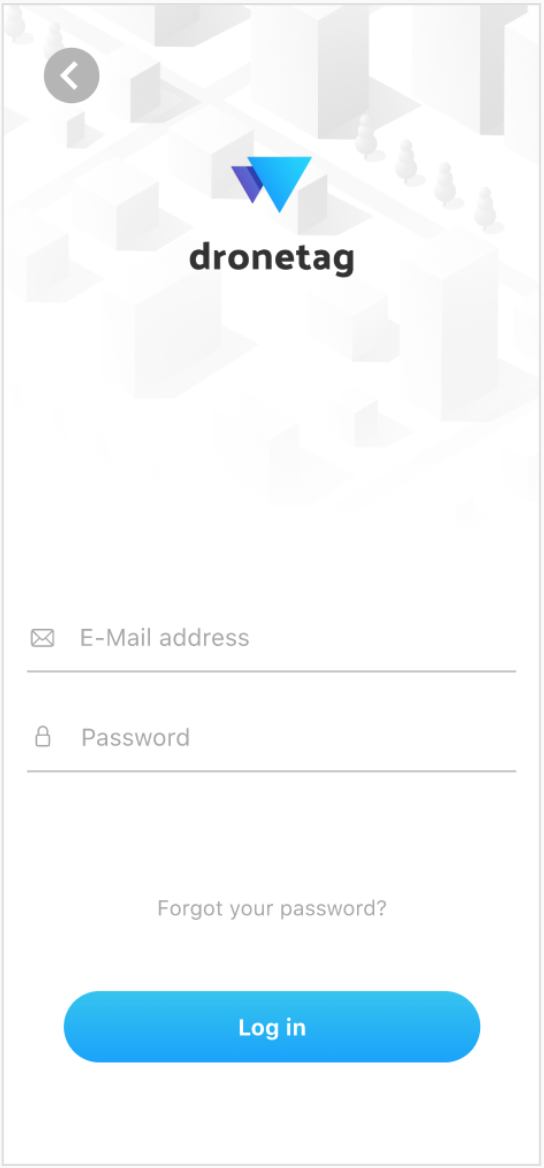
\includegraphics[width=.7\linewidth]{assets/user_interface_design/login/login_screen_log_in.png}
        \caption{[A11] Login screen, log in}
        \label{fig:login_screen_log_in}
    \end{minipage}%
    \hspace{.05\linewidth}
    \begin{minipage}{.45\textwidth}
        \centering
        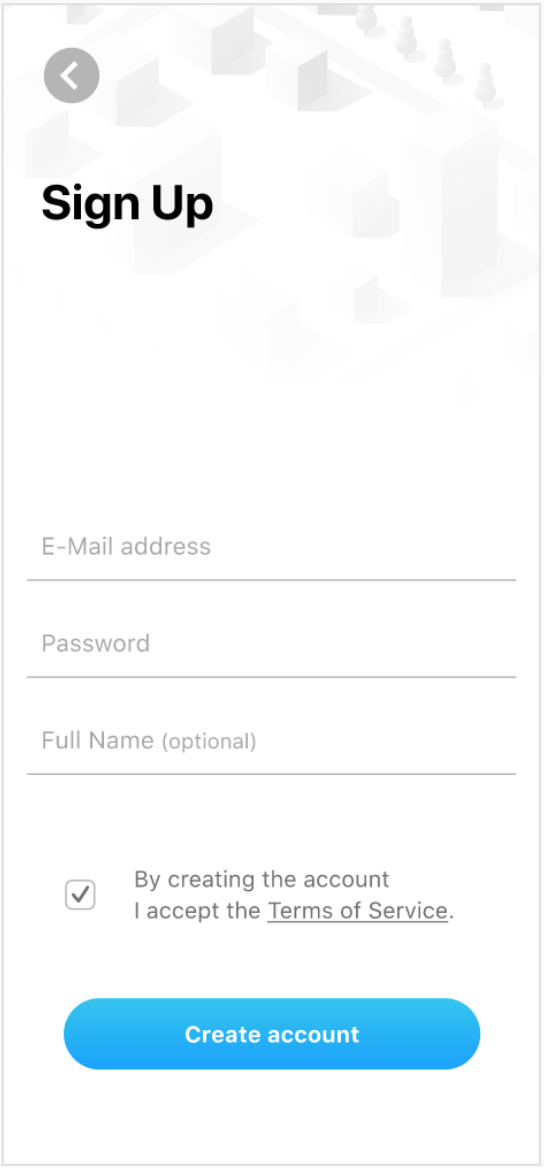
\includegraphics[width=.7\linewidth]{assets/user_interface_design/login/login_screen_sign_up.png}
        \caption{[A15] Dashboard, Place detail pinned}
        \label{fig:login_screen_sign_up}
    \end{minipage}
    \label{fig:login_screen_all}
\end{figure}


\subsection{Profile screens}\label{subsec:profile-screens}
The \textbf{Profile screen} (Figure \ref{fig:profile}) represents the menu of the application.
A user has granted access to his profile, management block, and he can see the set default aircraft and device.
Besides, if he belongs to an organization, it shows him the organization name and the button to switch the fleet mode.
My management container contains My Flights, My Devices and My Aircrafts buttons.

The \textbf{Profile detail} screen contains the user properties like the full name, phone number and country.
Also, it allows changing the user contact e-mail and password.


\begin{figure}
    \centering
    \begin{minipage}{.4\textwidth}
        \centering
        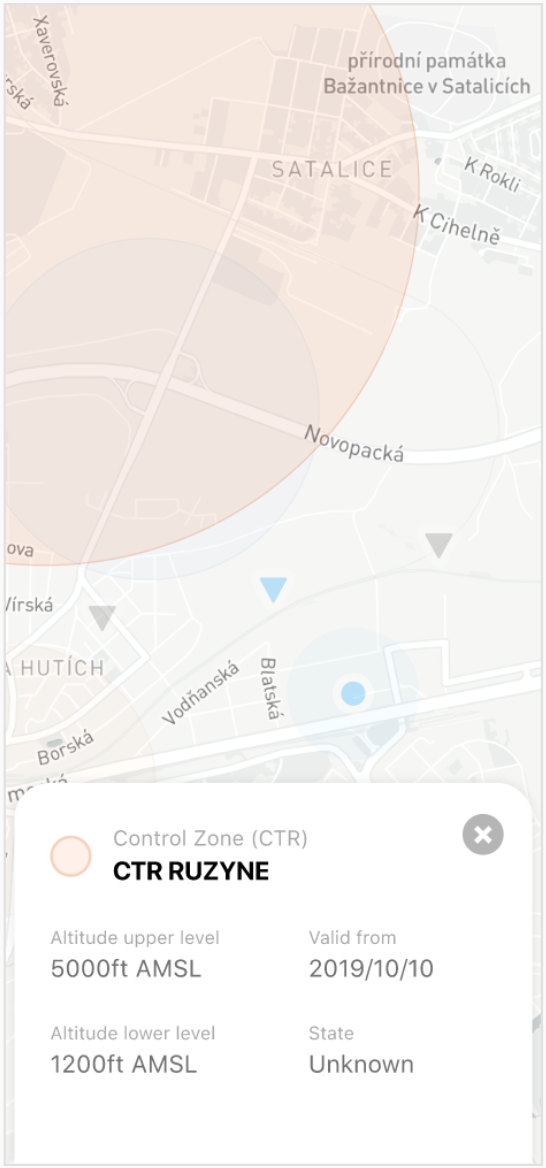
\includegraphics[width=.7\linewidth]{assets/user_interface_design/dashboard/dashboard_zone_detail.png}
        \caption{Dashboard, Zone detail}
        \label{fig:dashboard_zone_detail}
    \end{minipage}%
    \hspace{.05\linewidth}
    \begin{minipage}{.4\textwidth}
        \centering
        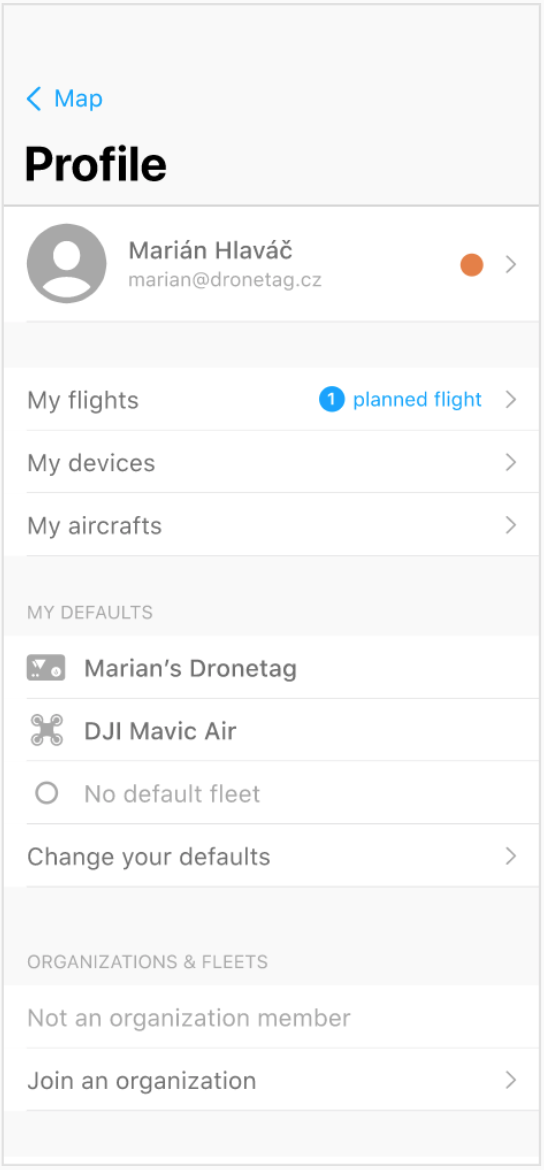
\includegraphics[width=.7\linewidth]{assets/user_interface_design/profile/profile.png}
        \caption{Profile}
        \label{fig:profile}
    \end{minipage}
    \label{fig:profile_all}
\end{figure}


\subsection{Device Screens}\label{subsec:device-screens}
The \textbf{Devices screen} (Figure~\ref{fig:devices}) will be showed after users click on My Devices button in the \textbf{Profile screen}.
This screen contains a list of registered Dronetag devices.
Also, here users can add a new device which bought via Add button.
Add button redirects the users to the \textbf{Device registration screen}.

The \textbf{Device screen} contains all information about the given device, including those which broadcasts in real--time.
Users can set the device as default or set the device preferences by their own needs here.

The \textbf{Device registration screen} is for registration of a new device that the users bought.
It contains two text fields for typing - a serial number, and an optional name for better identification.
After successful registration, the users are redirected to the \textbf{Devices screen}.


\subsection{Aircraft screens}\label{subsec:aircraft-screens}
\textbf{Aircrafts screen} contains a list of added aircrafts.
In addition, a user can add a new drone view Add button.
A user will get to this screen from Profile screen after the click to the My Aircrafts button.

\textbf{Aircraft screen} is for display the detail of an aircraft.
Simultaneously, it is used for adding new aircraft.
A user will get to it after choose a one from the list in \textbf{Aircrafts screen}.
This screen contains a form with four text fields:
\begin{itemize}
    \item the first is for type name,
    \item the second is for type UAS Operator ID what identify a person that has permission to flight with drones and passed the pilot exams,
    \item the third and four is for choosing the vendor and its model, and
    \item the last one is for setting the weight of aircraft
\end{itemize}


\subsection{Flight screens}\label{subsec:flight-screens}
%todo: add text


\begin{figure}
    \centering
    \begin{minipage}{.45\textwidth}
        \centering
        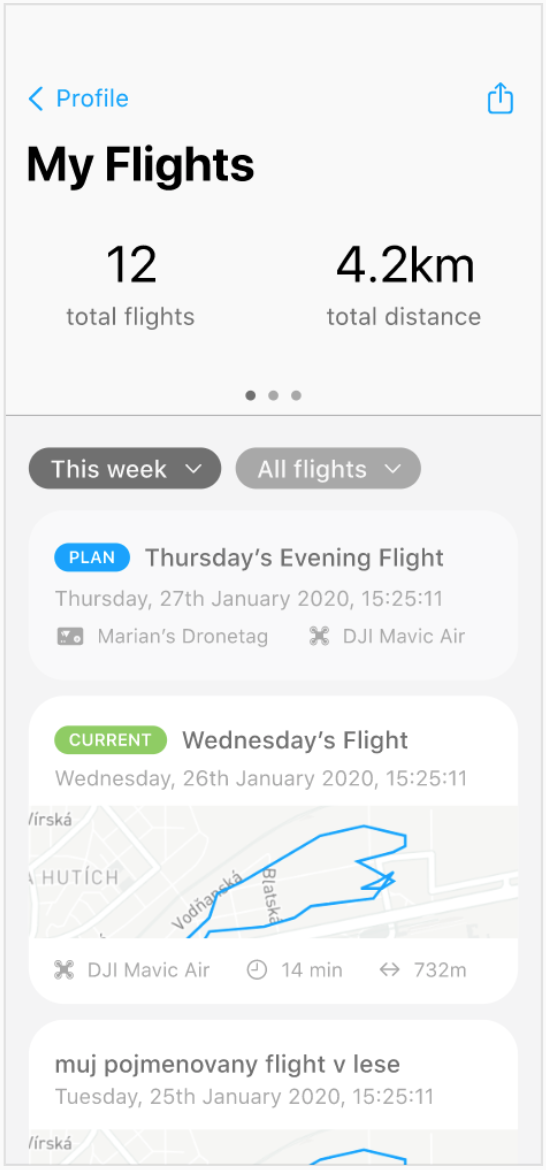
\includegraphics[width=.7\linewidth]{assets/user_interface_design/flight/flights.png}
        \caption{[A50] Flights}
        \label{fig:flights}
    \end{minipage}%
    \hspace{.05\linewidth}
    \begin{minipage}{.45\textwidth}
        \centering
        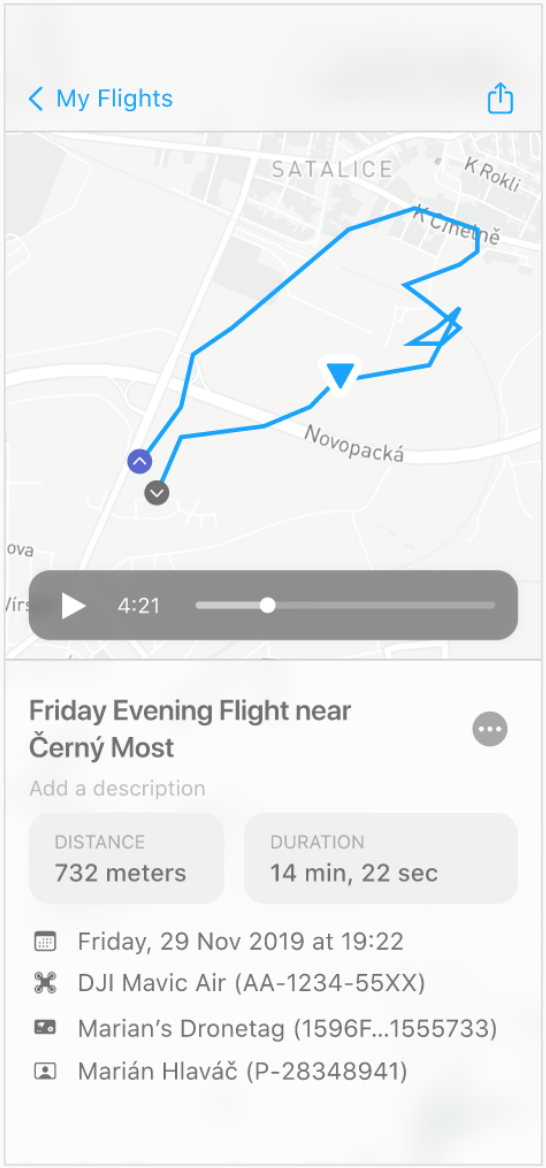
\includegraphics[width=.7\linewidth]{assets/user_interface_design/flight/flight_detail.png}
        \caption{[A51] Flight Detail}
        \label{fig:flight_detail}
    \end{minipage}
    \label{fig:flight_all}
\end{figure}

\begin{figure}
    \centering
    \begin{minipage}{.45\textwidth}
        \centering
        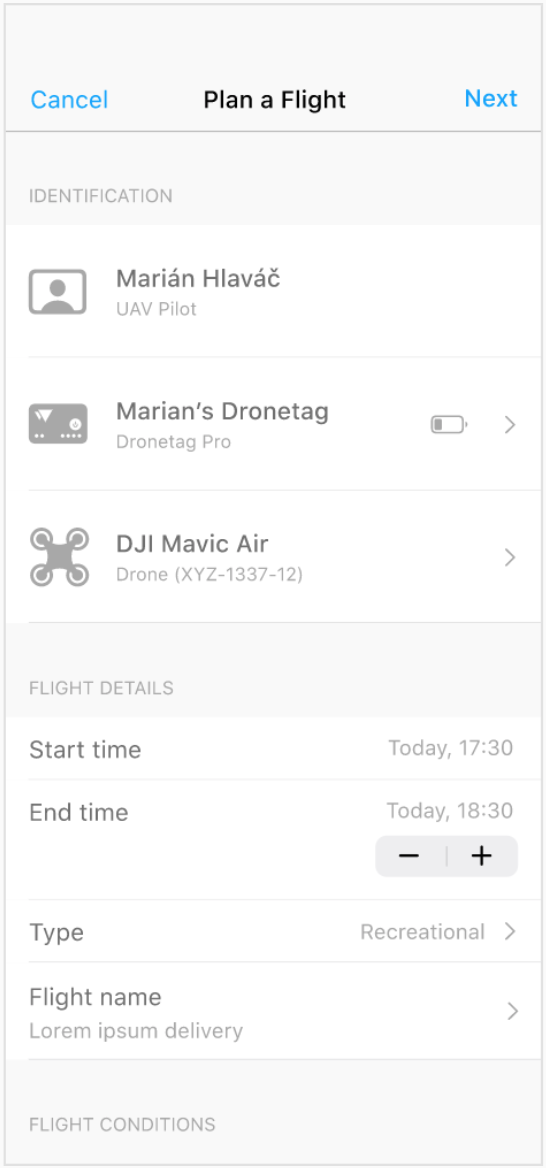
\includegraphics[width=.7\linewidth]{assets/user_interface_design/flight/plan_a_flight_step_1.png}
        \caption{[A33] Plan a Flight - Step 1}
        \label{fig:plan_a_flight_1}
    \end{minipage}%
    \hspace{.05\linewidth}
    \begin{minipage}{.45\textwidth}
        \centering
        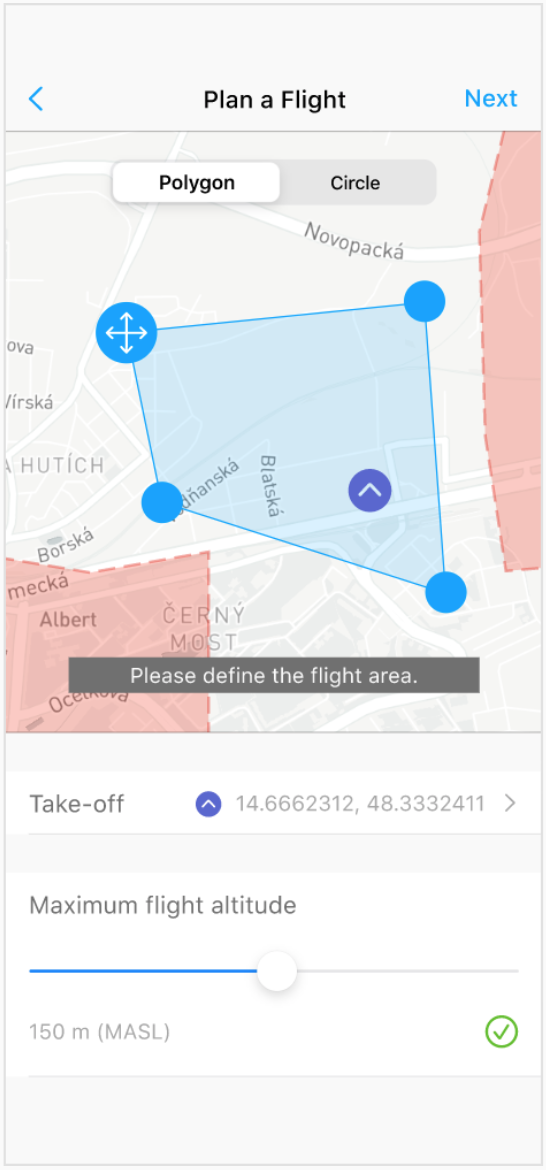
\includegraphics[width=.7\linewidth]{assets/user_interface_design/flight/plan_a_flight_step_2.png}
        \caption{[A34] Plan a Flight - Step 2}
        \label{fig:plan_a_flight_2}
    \end{minipage}
    \label{fig:plan_a_flight_all}
\end{figure}

\begin{figure}
    \centering
    \begin{minipage}{.45\textwidth}
        \centering
        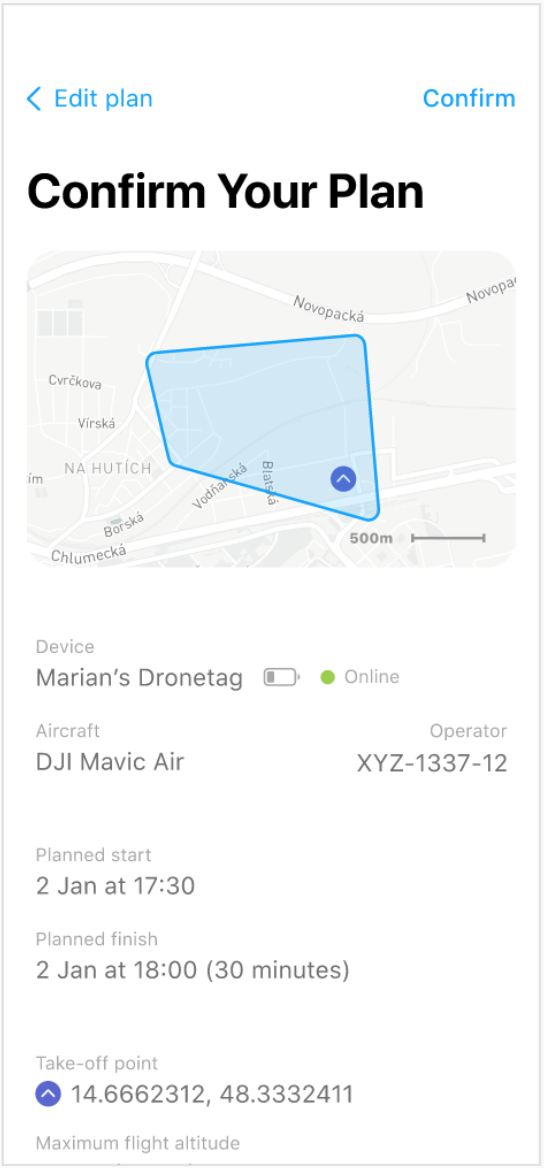
\includegraphics[width=.7\linewidth]{assets/user_interface_design/flight/plan_a_flight_step_3.png}
        \caption{[A35] Plan a Flight - Step 3}
        \label{fig:plan_a_flight_3}
    \end{minipage}%
    \hspace{.05\linewidth}
    \begin{minipage}{.45\textwidth}
        \centering
        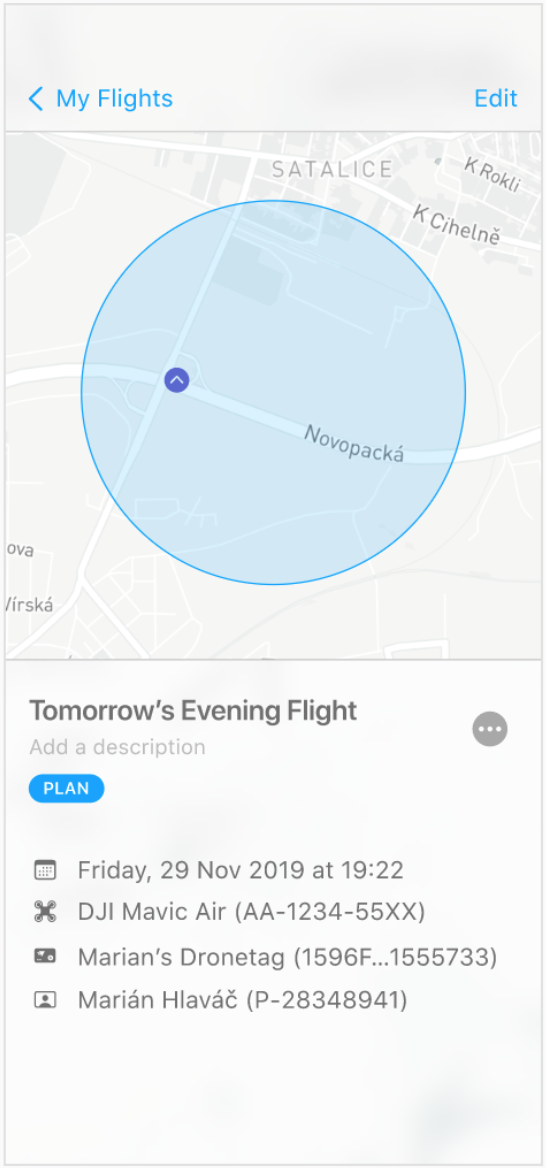
\includegraphics[width=.7\linewidth]{assets/user_interface_design/flight/flight_plan.png}
        \caption{[A52] Flight plan}
        \label{fig:flight_plan}
    \end{minipage}
    \label{fig:plan_a_flight_all_2}
\end{figure}

\begin{figure}
    \centering
    \begin{minipage}{.45\textwidth}
        \centering
        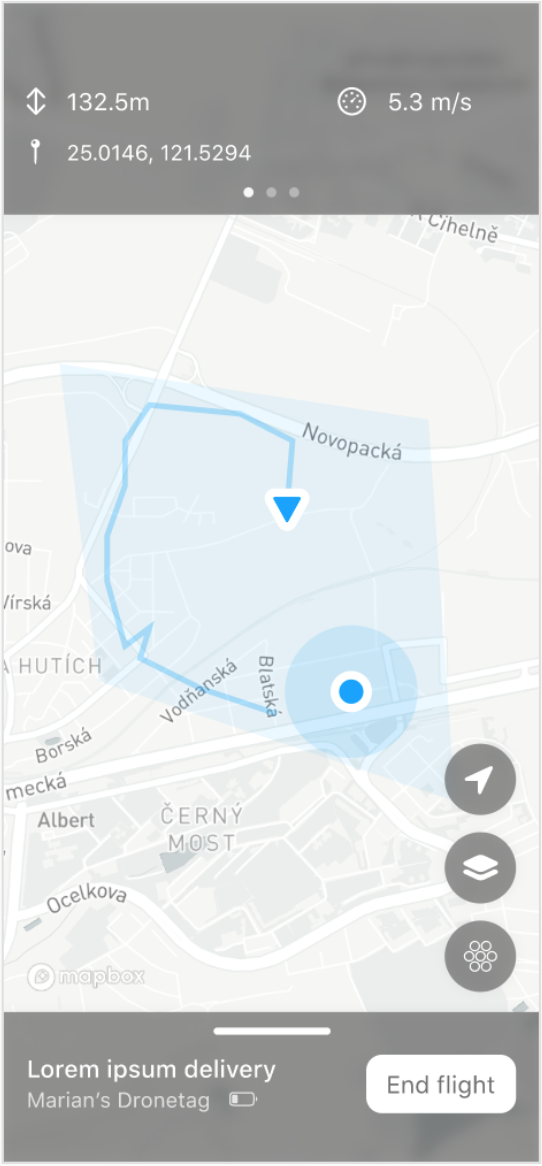
\includegraphics[width=.7\linewidth]{assets/user_interface_design/flight/in_flight.png}
        \caption{[A30] In-Flight}
        \label{fig:in_flight}
    \end{minipage}%
    \hspace{.05\linewidth}
    \begin{minipage}{.45\textwidth}
        \centering
        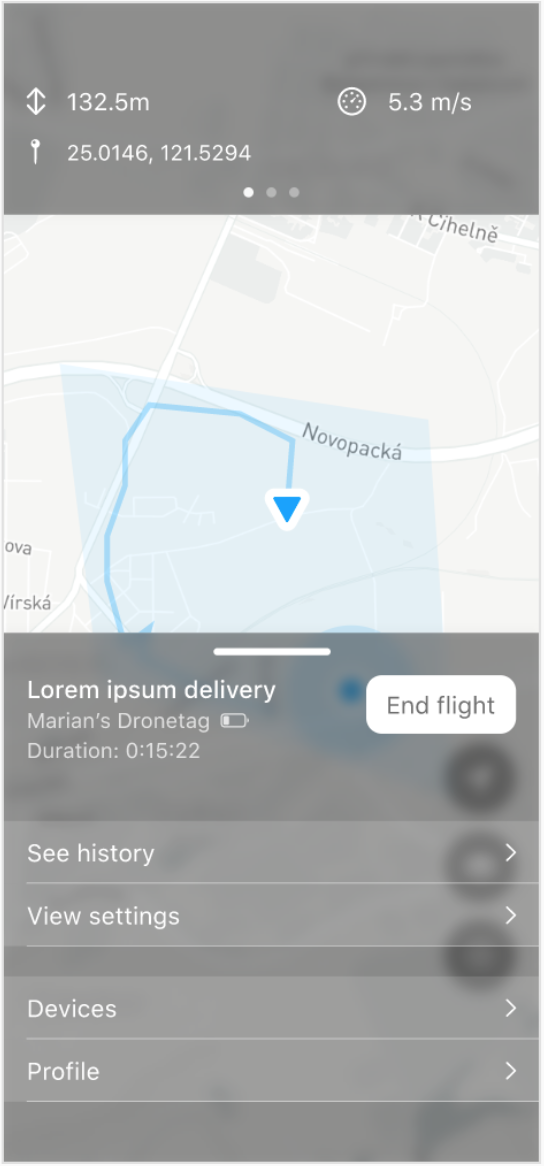
\includegraphics[width=.7\linewidth]{assets/user_interface_design/flight/in_flight_pulled_up.png}
        \caption{[A31] In-Flight, Pulled up}
        \label{fig:in_flight_pulled_up}
    \end{minipage}
    \label{fig:in_flight_all}
\end{figure}



\subsection{Search screen}\label{subsec:search-screen}
\textbf{Opened Search screen} (Figure \ref{fig:opened_search}) is the first what a user see when he clicks on the Search button in \textbf{Dashboard}.
It shows recent results that user has searched at the last time.
The result can be a drone, aircraft, place or zone.

If a user uses \textbf{Search text field} and type a text string, it will show to him a result with an icon for better identification (Figure \ref{fig:search_results}).
If a user choose an item in the list of results, it redirects him to either to \textbf{Aircraft detail} or \textbf{Device detail}, or even a place in the map in \textbf{Dashboard}.
After choosing that item, it will appear in the list of \textbf{Recent} results.

\begin{figure}
    \centering
    \begin{minipage}{.45\textwidth}
        \centering
        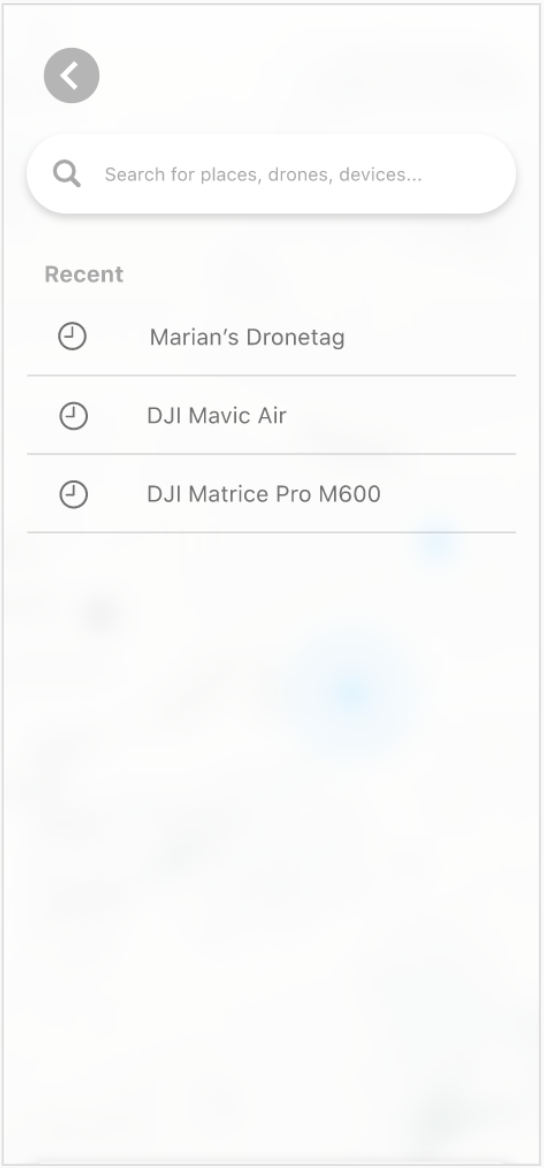
\includegraphics[width=.7\linewidth]{assets/user_interface_design/search/opened_search.png}
        \caption{[A60] Opened Search}
        \label{fig:opened_search}
    \end{minipage}%
    \hspace{.05\linewidth}
    \begin{minipage}{.45\textwidth}
        \centering
        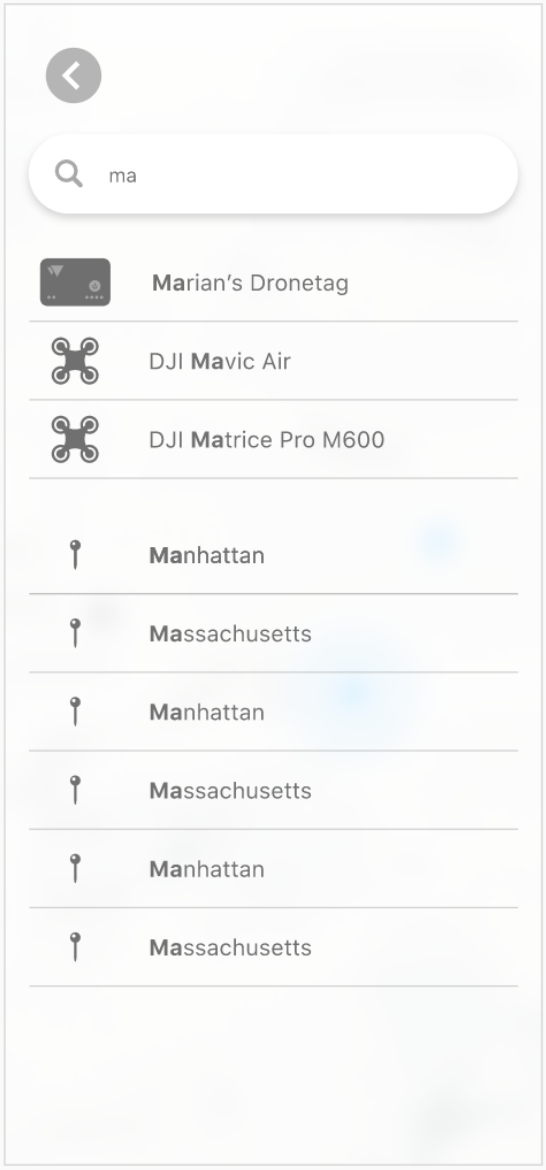
\includegraphics[width=.7\linewidth]{assets/user_interface_design/search/search_results.png}
        \caption{[A15] Search results}
        \label{fig:search_results}
    \end{minipage}
    \label{fig:search_all}
\end{figure}



\section{Usability testing}\label{sec:usability-testing}
In the User interface design cycle is the usability testing phase.
This phase involves testing with user who gets instruction by a scenario, and the task is to do it in his natural way.
The main purpose of this testing is detection of bad design elements and determination of the arrangement mistakes.
The elements can be arranged in a screen, part of a screen, menu or drop-down menu.
It depends on the purpose of concrete used application.

At first, we designed the Hi-fi prototype by the concurrent applications and we tried to learn from their design mistakes.
We had to decide if it is better to place a sliding panel with advisories on Dashboard or an animated button for a flight planning, how should look the profile menu screen and its icon or if it is useful to pin a place into the map.
After that we have organized the usability testing with common people who could be our potential customers.

During the testing we were detecting a few essential mistakes in the design.
They are closely described in following subsection Results \ref{subsec:results}.

\subsection{Results}\label{subsec:results}
We have tested with 6 users.
One of them was from Faculty of transportation sciencies, the others were my colleagues from Faculty of information technology.
Many of them were bachelor students, so it means they are between 20 and 25 of age.
The Faculty of transportation sciences' student gave me an insight what would expect a user with flight knowledge.
He describes me how should behave the map on the Dashboard and how I understand various map layers and flight levels.
My Faculty's colleagues were in the role of common users and helped me to understand what they expect of the used elements in the screens.

\subsection{Main mistakes in UI design}\label{subsec:main-mistakes-in-ui-design}
Během uživatelského testování jsme přišli na zajímavé poznatky, které jsou popsané v této části.
Některé jsme očekávali.
Některé nás naopak překvapili a donutili zvážit změnu v uživatelském rozhraní.
Například jsme zjistili, že:
\begin{enumerate}
    \item pro uživatele není přiliš intuitivní očekávat od Search buttonu vyhledávání dronů a devices.
    Očekává od toho pouze hledání místa, jelikož je součástí Dashboardu kde je hlavním prvkem mapa.
    \item není hned zřejmé, že panel dole se dá vytáhnout.
    To je také jedním z důvodů, proč jsme pro zatím sliding up panel with advisories vynechali.
    Ten druhý je, že pro zatím není známa a schválená legislativa a neustále se formuje.
    \item přiřazení konkrétního dronu k zařízení není příliš užitečně.
    Vhodnější je umožnit uživateli nastavit si default device a default drone a při plánování letu mu jej dovolit změnit.
    \item uživatel uvítá možnost hýbat s mapou v In-flight modu.
\end{enumerate}
Tyto poznatky měly velký dopad na to, že jsme nějaké screeny změnili tak, aby byly blížší vnímání uživatele.
